\documentclass[border=2pt]{standalone}
\usepackage{tikz}
\usetikzlibrary{positioning,calc,arrows.meta}
\begin{document}
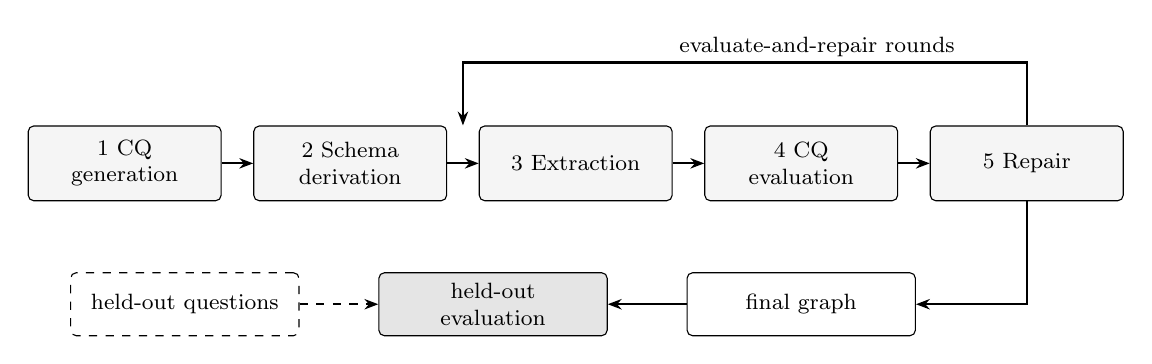
\begin{tikzpicture}[
  font=\footnotesize,
  stage/.style={draw, rounded corners=2pt, minimum width=2.45cm, minimum height=0.95cm, align=center, fill=black!4},
  side/.style={draw, rounded corners=2pt, minimum width=2.9cm, minimum height=0.8cm, align=center},
  arr/.style={-{Stealth[length=5pt]}, thick}]
  \node[stage] (s1) {1 CQ\\generation};
  \node[stage, right=0.4cm of s1] (s2) {2 Schema\\derivation};
  \node[stage, right=0.4cm of s2] (s3) {3 Extraction};
  \node[stage, right=0.4cm of s3] (s4) {4 CQ\\evaluation};
  \node[stage, right=0.4cm of s4] (s5) {5 Repair};
  \draw[arr] (s1) -- (s2);
  \draw[arr] (s2) -- (s3);
  \draw[arr] (s3) -- (s4);
  \draw[arr] (s4) -- (s5);
  \coordinate (top) at ($(s2.north)!0.5!(s3.north)$);
  \draw[arr] (s5.north) -- ++(0,0.8) -| (top);
  \node[above=0.75cm of s4, xshift=0.2cm] {evaluate-and-repair rounds};
  \node[side, below=0.9cm of s4] (fin) {final graph};
  \draw[arr] (s5.south) |- (fin.east);
  \node[side, left=1.0cm of fin, fill=black!10] (eval) {held-out\\evaluation};
  \draw[arr] (fin) -- (eval);
  \node[side, dashed, left=1.0cm of eval] (hq) {held-out questions};
  \draw[arr, dashed] (hq) -- (eval);
\end{tikzpicture}
\end{document}
